\section{Urządzenie lokalizujące}
\lstset{language=C}

Urządzenie to stanowi trzon całego systemu i to na nie spada największy ciężar funkcjonalny. Do jego zadań należą:

\begin{itemize}
\item Wykrywanie ruchu pojazu
\item Alarmowe powiadamianie właściciela w przypadku nieautoryzowanego przemieszczenia pojazdu
\item Pobieranie próbek lokalizacji, prędkości, przyspieszenia pojazdu po wykryciu ruchu i gromadzenie ich na zdalnym serwerze
\item Analiza stylu jazdy kierowcy
\item Wysyłanie poprzez SMS lokalizacji pojazdu na żądanie użytkownika
\end{itemize}

Duża liczba zadań do wykonania przez procesor i konieczność wywoływania ich po ściśle określonym czasie, spowodowała, że niezbędnym stało się wprowadzenie modułu planisty. Stanowi on bardzo prostą funkcjonalność, bez możliwości wywłaszczania zadań i zmiany kontekstu, więc nie wprowadza funkcjonalności wielowątkowości znanej z pełnopranych systemów operacyjnych. Jego celem jest zakolejkowanie zadań i oznaczenie ich jako do wykonania, po wymaganym czasie. Kod służący kolejkowania przedstawiono na listingu \ref{listing_scheduler_add}. Na listingu \ref{listing_scheduler_check} przedstawiono funkcję, która wywyływana jest cyklicznie co 10 ms w przerwaniu od energooszczędnego timera, służącą do oznaczania zadań, które można już wykonać. Na ostatnim listingu, oznaczonym numerem  \ref{listing_scheduler_exec}, przedstawiono funkcję wykonującą zadania. Ograniczeniem funkcjonalnym jest tutaj fakt, iż żadne z zadań nie może przyjmować argumentów, ani zwracać wartości. 
\clearpage

\begin{lstlisting}[label=listing_scheduler_add, caption=Funkcja do kolejkowania zadań]

scheduler_error_code_e SchedulerAddOperation(void (*callback)(void),
	 										volatile	uint32_t timeMsFromNow,
	 										volatile uint8_t* taskIndex,
	 										bool isCyclic){
    scheduler_entry_t entry;

    // Just safe guard not to miss the time
    if (timeMsFromNow < 2)
    {
        timeMsFromNow = 2;
    }

    for (uint8_t i=0; i< SCHEDULER_BUFFER_SIZE; ++i)
    {
        if (_scheduleBuffer[i].isInProgress == false)
        {
            entry.isInProgress = true;
            entry.isTimedOut = false;
            entry.callback = callback;
            entry.timePeriodMs = timeMsFromNow;
            entry.triggerTime = scheduler_current_time_ms + timeMsFromNow;
            entry.isCyclic = isCyclic;
            memcpy(&_scheduleBuffer[i], &entry, sizeof(scheduler_entry_t));
            if (taskIndex != NULL)
                *taskIndex = i;
            return E_SCHEDULER_OK;
        }
    }

    return E_SCHEDULER_NO_RESOURCES;
}
\end{lstlisting}

\clearpage
\begin{lstlisting}[label=listing_scheduler_check, caption=Funkcja do sprawdzania czy nie należy wykonań zadania]

scheduler_error_code_e SchedulerCheckOperations(){
    scheduler_current_time_ms += 10;
    for (uint8_t i=0; i< SCHEDULER_BUFFER_SIZE; ++i)
    {
        if (_scheduleBuffer[i].isInProgress == true &&
            _scheduleBuffer[i].triggerTime <= scheduler_current_time_ms)
        {
            // If it is cyclic task - reschedule the next cycle
            if (_scheduleBuffer[i].isCyclic)
            {
                _scheduleBuffer[i].triggerTime = scheduler_current_time_ms 
                +_scheduleBuffer[i].timePeriodMs;
            }

            _scheduleBuffer[i].isTimedOut = true;
        }
    }

    return E_SCHEDULER_OK;
}
\end{lstlisting}


\begin{lstlisting}[label=listing_scheduler_exec, caption=Funkcja do wykonywania zadań]

scheduler_error_code_e ScheduleExecutePendingOperations(){
    for (uint8_t i=0; i< SCHEDULER_BUFFER_SIZE; ++i)
    {
        if (_scheduleBuffer[i].isInProgress == true && 
        		_scheduleBuffer[i].isTimedOut == true)
        {
            if (_scheduleBuffer[i].isCyclic == false)
            {
                _scheduleBuffer[i].isInProgress = false;
            }
            _scheduleBuffer[i].callback();
            _scheduleBuffer[i].isTimedOut = false;
        }
    }

    return E_SCHEDULER_OK;
}

\end{lstlisting}

Główny cykl działania urządzenia został przedstawiony na rysunku \ref{fig:image_soft_mainboard_main_alghoritm}.

\begin{figure}[H]
	\centering
	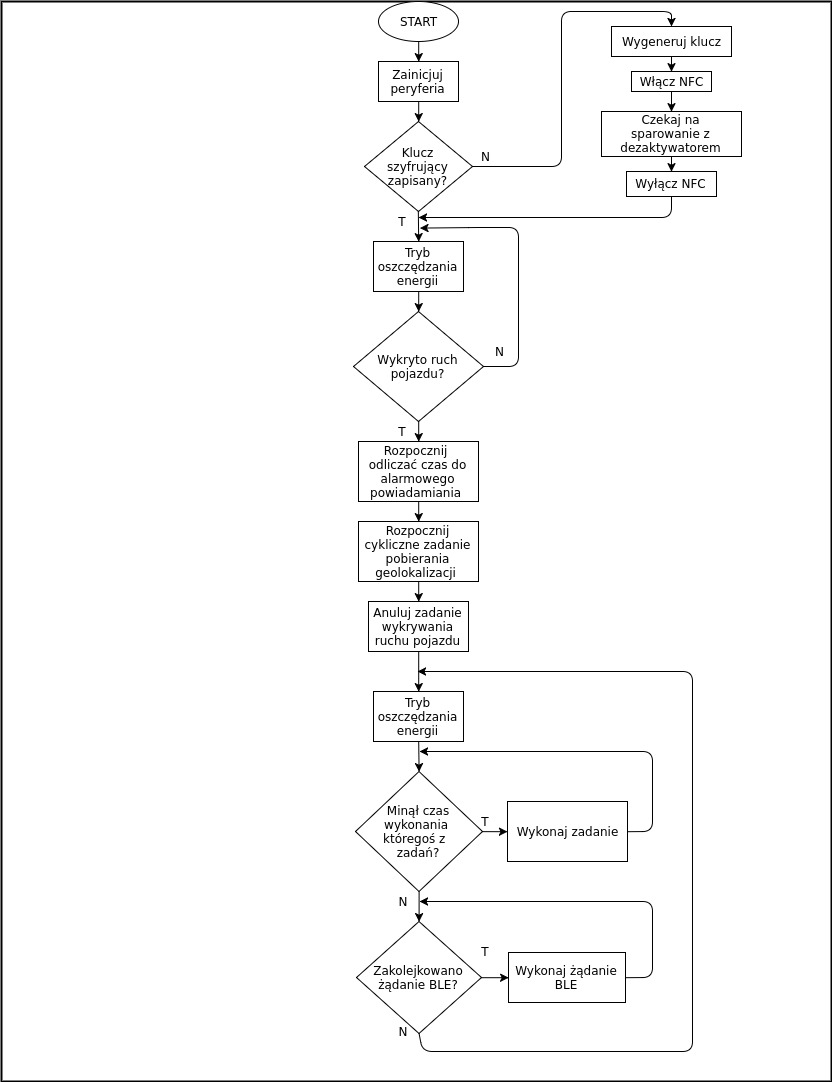
\includegraphics[width=16cm]{img/software/mainboard/Tracking_alghoritm.jpg}
	\caption{Główny algorytm działania urządzenia. 
	\\Źródło: Twórczość własna}
	\label{fig:image_soft_mainboard_main_alghoritm}
\end{figure}

Jak widać na rysunku \ref{fig:image_soft_mainboard_main_alghoritm}, po uruchomieniu i zainicjalizowaniu peryferiów i modułów na płytce, mikrokontroler dokonuje sprawdzenia czy wygenerowany został klucz szyfrujący, służacy do zabezpieczenia komunikacji z dedykowanym urządzeniem deaktywującym. Jeśli klucza nie ma, oznacza to, że urządzenie nie zostało jeszcze sparowane. Wówczas, włączony zostaje układ NFC, procesor wchodzi w tryb oszczędzania energii w trakcie oczekiwania na parowanie, a całe urządzenie staje się nieoperacyjne, dopóki nie zostanie powiązane z modułem deaktywującym. Gdy zostanie to zrobione, moduł NFC zostaje wyłączony (i nie jest używany aż do momentu powrotu do ustawień fabrycznych), a mikrokontroler wchodzi w tryb oszczędzania energii w oczekiwaniu na nadchodzące zadania.

Pierwszym z nich jest wykrywanie ruchu pojazdu. Zostało to zrealizowane poprzez wykorzystanie funkcjonalności akcelerometru - wybudzenia w razie wykrycia przyspieszenia powyżej progu wynoszącego 1.2 $\frac{m}{s^2}$ i utrzymującego się przez więcej niż 1 sekundę. Jest on cykliczne, co 5 sekund, odpytywany, czy nie nastąpiło takie zdarzenie. Jeśli nie nastąpiło, cykl się powtarza. Jeśli wykryto ruch, zadanie okresowego sprawdzania ruchu jest wyłączane, natomiast do kolejki zadań ładowane są 3 najważniejsze z punktu widzenia całego systemu - zadanie alarmu, skanowania w poszukiwaniu \textit{Key Tag'a} oraz cyklicznego pobierania próbek lokalizacji. Pierwsze z nich, stanowi zegar, który odlicza 30 sekund. Jeśli w tym czasie, alarm zostanie deaktywowany poprzez nawiązanie połączenia z urządzeniem dezaktywującym i nadanie odpowiedniego komunikatu, wówczas zadanie zostaje anulowane i jedynym cyklicznym zadaniem jest próbkowanie lokalizacji. W przeciwnym razie, uruchamiane jest zadanie cyklicznego, co 10 minutowego powiadamiania właściciela o lokalizacji pojazdu poprzez wiadomości SMS. Okres ten został dobrany w ten sposób, aby nie wyczerpać za szybko śródków na koncie karty SIM, użytej w module, a przy tym uzyskać rozsądną częstotliwość wysyłania SMS'ów. Zadanie to można anulować, w przypadku fałszywego alarmu, wysyłając odpowiednią komendę poprzez SMS z numeru właściciela. 

Ponadto, równolegle, niezależnie od tego czy alarm został deaktywowany czy nie, uruchamiane jest zadanie cyklicznego pobierania próbek lokalizacji. Okres wynosi 10 sekund i w momencie próbkowania pobierane są dane takie jak:

\begin{itemize}
\item Status lokalizacji (brak sygnału z satelitów, lokalizacjia wyznaczona)
\item Lokalizacja pojazdu
\item Prędkość pojazdu
\item Średnie przyspieszenie pojazdu z okresu pomiędzy próbkami
\item Azymut ruchu
\item Ocena jazdy z okresu pomiędzy próbkami
\item Parametr HDOP informujący o dokładności wyznaczenia lokalizacji (idealnie, wartość mniejsza od 1)
\item Liczba satelitów z których odebrano sygnał
\item Czas pobrania próbki
\end{itemize}

Na rysunku \ref{fig:image_soft_mainboard_control_flow} przedstawiono diagram interakcji, ktory pokazuje przeływ sterowania pomiędzy zadaniami. 



\begin{figure}[H]
	\centering
	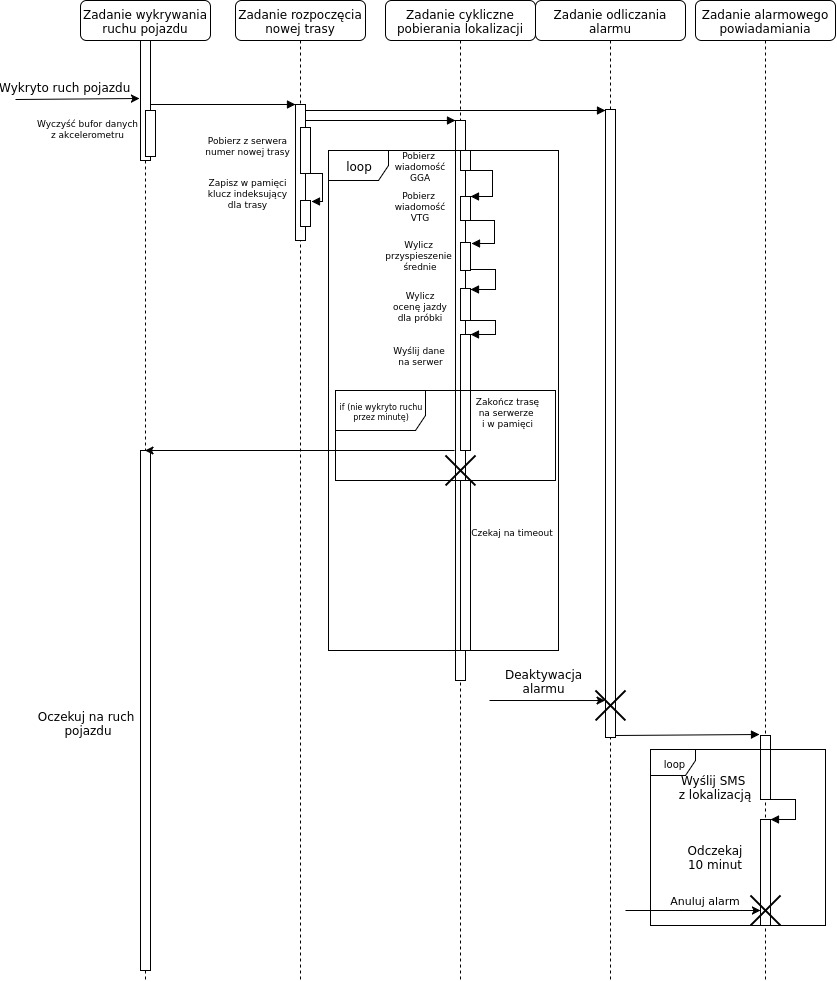
\includegraphics[width=17cm]{img/software/mainboard/MainBoardStartTracking.jpg}
	\caption{Przepływ sterowania w przypadku wykrycia ruchu pojazdu. 
	\\Źródło: Twórczość własna}
	\label{fig:image_soft_mainboard_control_flow}
\end{figure}